% !TeX root = ../../Skript.tex
\cohead{\Large\textbf{Normalengleichungen}}
\fakesubsection{Normalengleichungen bestimmen}
Eine Normale an eine Funktion ist eng mit der Tangenten verwandt. Während eine Tangente am Berührpunkt die gleiche Steigung wie die Funktion hat, schneidet eine Normale die Funktion senkrecht. Damit eine Gerade \(n(x)=mx+b\) eine Normale an der Stelle \(x_0\) an das Schaubild einer Funktion \(f(x)\) ist, müssen 2 Bedingungen erfüllt sein:

\iftoggle{qrcode}{\setlength{\qrheight}{2.5cm}}{\setlength{\qrheight}{0cm}}%
\begin{minipage}{\linewidth}
    \begin{minipage}{\linewidth-\qrheight}
    \begin{tcolorbox}[width=\linewidth]

        \bigskip

	   \textcolor{loestc}{Die Normalen an der Stelle \(x_0\) muss senkrecht zur Funktion stehen:
		\[m\cdot f'(x_0)=-1\]}
    \end{tcolorbox}%
    \end{minipage}%
    \iftoggle{qrcode}{\begin{minipage}{\qrheight}
        \href{https://www.geogebra.org/m/faavja2d}{
\includegraphics[height=\qrheight]{\ableitung/pics/NormalenQR.png}}%
    \end{minipage}}{}%
\end{minipage}%
\begin{tcolorbox}

    \bigskip

	\textcolor{loestc}{Die Funktionswerte der Normalen und der Funktion an der Stelle \(x_0\) müssen gleich sein:
		\[n(x_0)=f(x_0)\]}
\end{tcolorbox}
Beispiel: Bestimme die Normale an die Funktion \(f(x)=-\frac{1}{2}x^2-x+3\) an der Stelle \(x_0=1\).\vspace{0.5cm}
\begin{minipage}{\textwidth}
    \adjustbox{valign=t}{\begin{minipage}{0.5\textwidth+2ex}
		\begin{enumerate}
			\item Produkt der Steigungen muss -1 ergeben:

			\bigskip

            \bigskip

			\textcolor{loes}{\(f'(x)=-x-1\) und damit \(f'(1)=-2\)}

			\textcolor{loes}{Aus \(-2\cdot m_n = -1\) folgt, dass \(m_n=\frac{1}{2}\)}

            \bigskip

            \bigskip

			\item Gleiche Funktionswerte an der Stelle \(x_0=1\):

            \smallskip

			\begin{align*}
				\textcolor{loes}{n(1)}&\textcolor{loes}{=f(1)}\\
				\textcolor{loes}{\frac{1}{2}\cdot 1+b}&\textcolor{loes}{=-\frac{1}{2}\cdot 1^2-1+3}\\
				\textcolor{loes}{\frac{1}{2}+b}&\textcolor{loes}{=\frac{3}{2}\ \vert\ -\frac{1}{2}}\\
				\textcolor{loes}{b}&\textcolor{loes}{=1}
			\end{align*}


            \textcolor{loes}{Damit ergibt sich \(nn(x)=\frac{1}{2}x+1\)}
		\end{enumerate}
	\end{minipage}}%
    \adjustbox{valign=t, padding=2ex 0ex 0ex 0ex}{\begin{minipage}{0.5\textwidth-4ex}
		\centering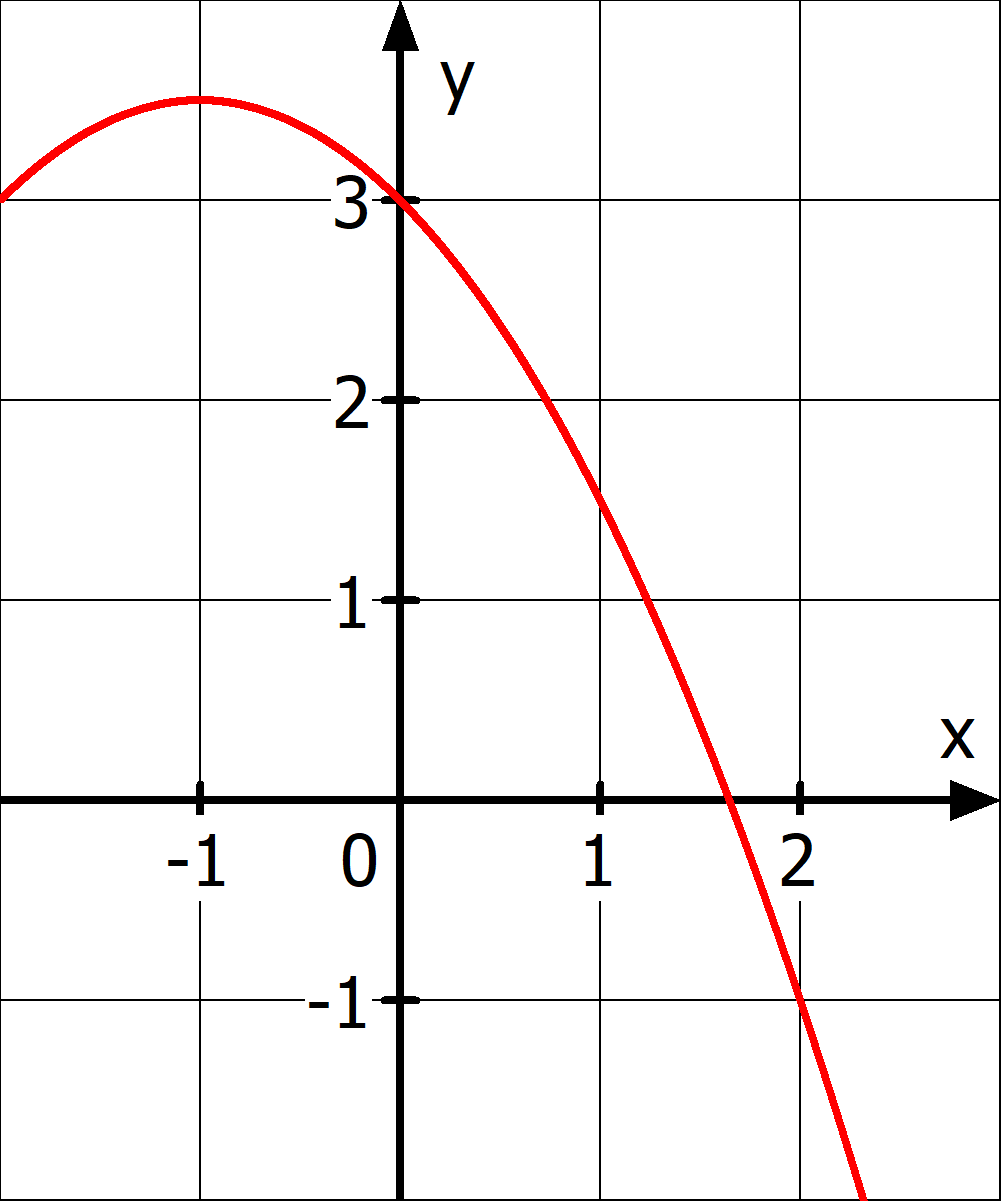
\includegraphics[width=\textwidth]{\ableitung/pics/normaleBsp.png}
	\end{minipage}}%
\end{minipage}\newpage
%%%%%%%%%%%%%%%%%%%%%%%%%%%%%%%%%%%%%%%%%%%%%%%%%%%%%%%%%%%%%%%%%%%%%%%%%%%%%%%%%%%%%%%%%%%%%%%%%%%%%%%
\begin{Exercise}[title={\raggedright Bestimme jeweils die Normalengleichung.}, label=normaleBestimmenA1]
	\begin{enumerate}[label=\alph*)]
		\item \(f(x)=-x^2+1\) an der Stelle \(x_0=-1\)
		\item \(f(x)=-1,5x^2+x\) an der Stelle \(x_0=2\)
		\item \(f(x)=x^3+2\) an der Stelle \(x_0=1\)
		\item \(f(x)=-2x^2+2x\) an der Stelle \(x_0=0\)
		\item \(f(x)=-0,25x^4+9x\) an der Stelle \(x_0=-3\)
		\item \(f(x)=\frac{3}{2}x^2-2x+1\) an der Stelle \(x_0=-3\)
		\item \(f(x)=x^3-2x^2+x\) an der Stelle \(x_0=\frac{2}{3}\)
		\item \(f(x)=\frac{1}{6}x^3-\frac{1}{2}x+3\) an der Stelle \(x_0=1\)
		\item \(f(x)=e^x\) an der Stelle \(x_0=-\ln(2)\)
		\item \(f(x)=3e^{-2x}\) an der Stelle \(x_0=\ln\left(3\right)\)
		\item \(f(x)=\frac{5}{8}x^4-\frac{5}{4}x^2-x\) an der Stelle \(x_0=-1\)
		\item \(f(x)=\frac{1}{2}x^2-3x+5\) an der Stelle \(x_0=-6\)
		\item \(f(x)=2e^{-3x}\) an der Stelle \(x_0=0\)
		\item \(f(x)=-\frac{3}{2}e^{0,5x}-3\) an der Stelle \(x_0=\ln(16)\)
		\item \(f(x)=-\frac{5}{16}x^4+\frac{7}{12}x^3+\frac{3}{4}x\) an der Stelle \(x_0=-1\)
	\end{enumerate}
\end{Exercise}
%%%%%%%%%%%%%%%%%%%%%%%%%%%%%%%%%%%%%%%%%
\begin{Answer}[ref=normaleBestimmenA1]

	\begin{enumerate}[label=\alph*)]
		\item \(n(x)=-\frac{1}{2}x-\frac{1}{2}\)
		\item \(n(x)=\frac{1}{5}x-\frac{22}{5}\)
		\item \(n(x)=-\frac{1}{3}x+\frac{10}{3}\)
		\item \(n(x)=-\frac{1}{2}x\)
		\item \(n(x)=-\frac{1}{36}x-\frac{142}{3}\)
		\item \(n(x)=\frac{1}{11}x+\frac{457}{22}\)
		\item \(n(x)=3x-\frac{52}{27}\)
		\item \(n(x)=-2x+\frac{8}{3}\)
		\item \(n(x)=-2x+\frac{1}{2}-\ln(4)\)
		\item \(n(x)=\frac{3}{2}x+\frac{1}{3}-\frac{3}{2}\ln(3)\)
		\item \(n(x)=x+\frac{11}{8}\)
		\item \(n(x)=\frac{1}{9}x+\frac{125}{3}\)
		\item \(n(x)=\frac{1}{6}x+2\)
		\item \(n(x)=\frac{1}{3}x-9-\frac{1}{3}\ln(16)\)
		\item \(n(x)=\frac{15}{4}x-\frac{153}{80}\)
	\end{enumerate}
\end{Answer}